
This section reports the results on $\PgU$ production in pp and
PbPb obtained from the yield extraction procedure described in Section
\ref{sec:Yields}.
First, single differential cross sections of $\PgU$ production in pp collisions are
reported in Section \ref{subsec:cspp}. Then, $\PgU$ invariant
yields in PbPb collisions divided by the %expected
 nuclear overlap
function \TAA\ are presented in Section \ref{subsec:csaa}. These
results are also formulated in terms of the nuclear modification
factor \RAA\ in order to reveal the suppression of $\PgUa$ and
$\PgUb$ 
as a function of the transverse momentum and rapidity.
%in bins of kinematic quantities. 
The updated
measurement of centrality-dependent suppression is reported in Section
\ref{subsec:raah}. Finally, the
results for the $\PgU$(3S) state are presented in Section \ref{sec:Y3S}. 

\subsection{Inclusive differential cross section of \texorpdfstring{$\PgU$}{Y} production in pp}
\label{subsec:cspp}
The differential quarkonium cross section as a function of $\pt$ and $y$ is determined from yields extracted in
Sections \ref{subsec:ptbins} and \ref{subsec:rapbins}, corrected for
acceptance and efficiency and luminosity. 
It is given by
\begin{eqnarray} 
\label{eq:cspt}
\dfrac{1}{\Delta y}\ \dfrac{\text{d}\sigma\left( pp\rightarrow \PgU(nS)X\right)}{\text{d}\pt} \cdot B_{\mu\mu} &=& \dfrac{1}{\Delta y \Delta \pt}\cdot\dfrac{1}{\mathcal{L}_{pp}}\cdot\dfrac{\NFitnS}{\alpha\ \varepsilon_{\rm pp} } \\
\label{eq:csrap}
\dfrac{\text{d}\sigma\left( pp\rightarrow
\PgU(nS)X\right)}{\text{d}y} \cdot B_{\mu\mu} &=&
\dfrac{1}{\Delta y}\cdot\dfrac{1}{\mathcal{L}_{pp}}\cdot\dfrac{\NFitnS} {\alpha\ \varepsilon_{\rm pp}} 
\end{eqnarray}
% 
where:
\begin{itemize}
\item{\NFitnS\ is the number of measured $\PgU$ decaying to
two muons, from the fit
to data;}
\item{$\alpha$ is the geometric acceptance, computed in Section
\ref{sec:Efficiency};}
\item{$\varepsilon_{\rm pp}$ is the dimuon trigger and reconstruction
efficiency, which differs from that of the PbPb set-up;}
\item{$\mathcal{L}_{pp}$ = (5.4 $\pm$ 0.2) pb$^{-1}$ is the integrated
luminosity of the pp sample;}
\item{$\Delta \pt$ and $\Delta y$ are the bin widths in $\pt$ and $y$, described in Section~\ref{subsec:ptbins} and~\ref{subsec:rapbins}, respectively. Note that in Eq.~(\ref{eq:cspt})}, the yields are integrated over the CMS rapidity acceptance ($|y|<2.4$, $\Delta y=4.8$).
\end{itemize}

The $\PgU$ pp cross sections are shown as
a function of $\pt$ in Figure \ref{fig:CSpppt} and as a function of
$|y|$ in Figure \ref{fig:CSpprap}. Tabulated results are reported in
Table \ref{tab:CSpppttab} and \ref{tab:CSppraptab}, respectively.
\vfill\newpage
%
\begin{figure}[ht]
\begin{centering}  
  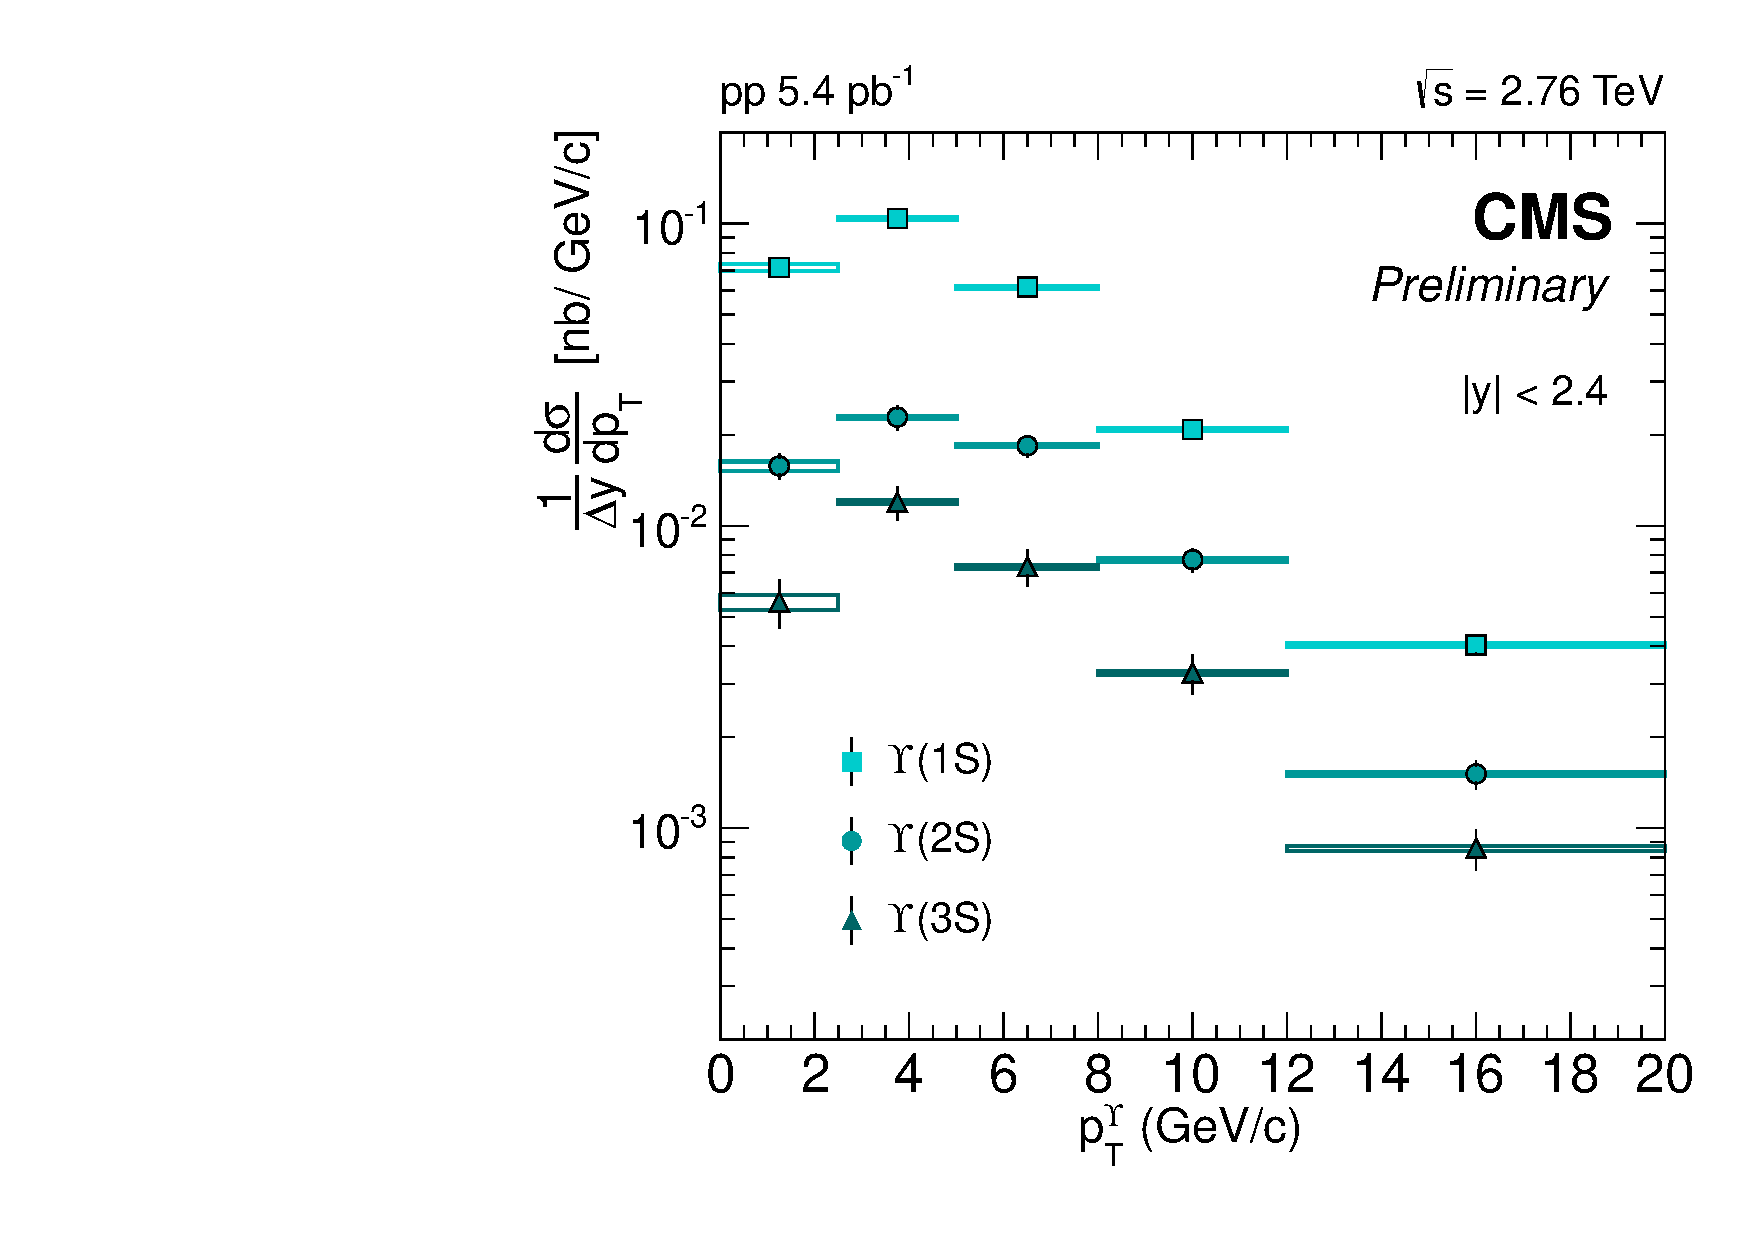
\includegraphics[width=0.7\textwidth]{Results/CS1S_ppPt.pdf}
  \caption{\PgUa, \PgUb, \PgUc\ production cross section in pp
  collisions as a function of $\pt$.}
  \label{fig:CSpppt} 
\end{centering}  
\end{figure}
%
\begin{table}[ht]
\begin{centering}
\begin{tabular}{|c|c|c|c|}                                      
\hline
pp, $|y| < $2.4 &  \multicolumn{3}{c}{$\frac{1}{\Delta y}\frac{d\sigma_{nS}}{d\pt}\cdot B_{\mu\mu}$ [nb $\cdot$ c/GeV]} \vline \\
\hline
%State
 &  $\PgUa$ & $\PgUb$ &  $\PgU$(3S) \\ 
\hline  %%[{\rm GeV}/c]
\pt  $<$ 2.5       & 0.0729$\pm$ 0.00248 $\pm$ 0.00206     &0.0158 $\pm$ 0.00153 $\pm$ 0.000551   & 0.00559 $\pm$ 0.00103 $\pm$ 0.000318  \\  
2.5 $<$ \pt $<$ 5  & 0.105$\pm$ 0.00343 $\pm$ 0.0014       &0.0229 $\pm$ 0.00217 $\pm$ 0.000244   & 0.012 $\pm$ 0.00158 $\pm$ 0.00017     \\   
5 $<$ \pt  $<$ 8   & 0.0626$\pm$ 0.00214 $\pm$ 0.000691    &0.0184 $\pm$ 0.00153 $\pm$ 0.0002     & 0.00733 $\pm$ 0.00105 $\pm$ 0.0001    \\  
8 $<$ \pt  $<$ 12  & 0.021$\pm$ 0.00098 $\pm$ 0.000261     &0.00773 $\pm$ 0.000698 $\pm$ 0.000113 & 0.00326 $\pm$ 0.000494 $\pm$ 5.37e-05 \\ 
12 $<$ \pt $<$ 20  & 0.00406$\pm$ 0.000247 $\pm$ 6.28e-05  &0.00151 $\pm$ 0.000167 $\pm$ 2.69e-05 & 0.000858 $\pm$ 0.000132 $\pm$ 1.69e-05\\

\hline
\end{tabular}
\caption{$\pt$-differential cross section in pp collisions. Listed
uncertainties are statistical (first) and systematic (second).}  
\label{tab:CSpppttab}
\end{centering}
\end{table}

\vfill\newpage
%
\begin{figure}[ht]
\begin{centering}       
  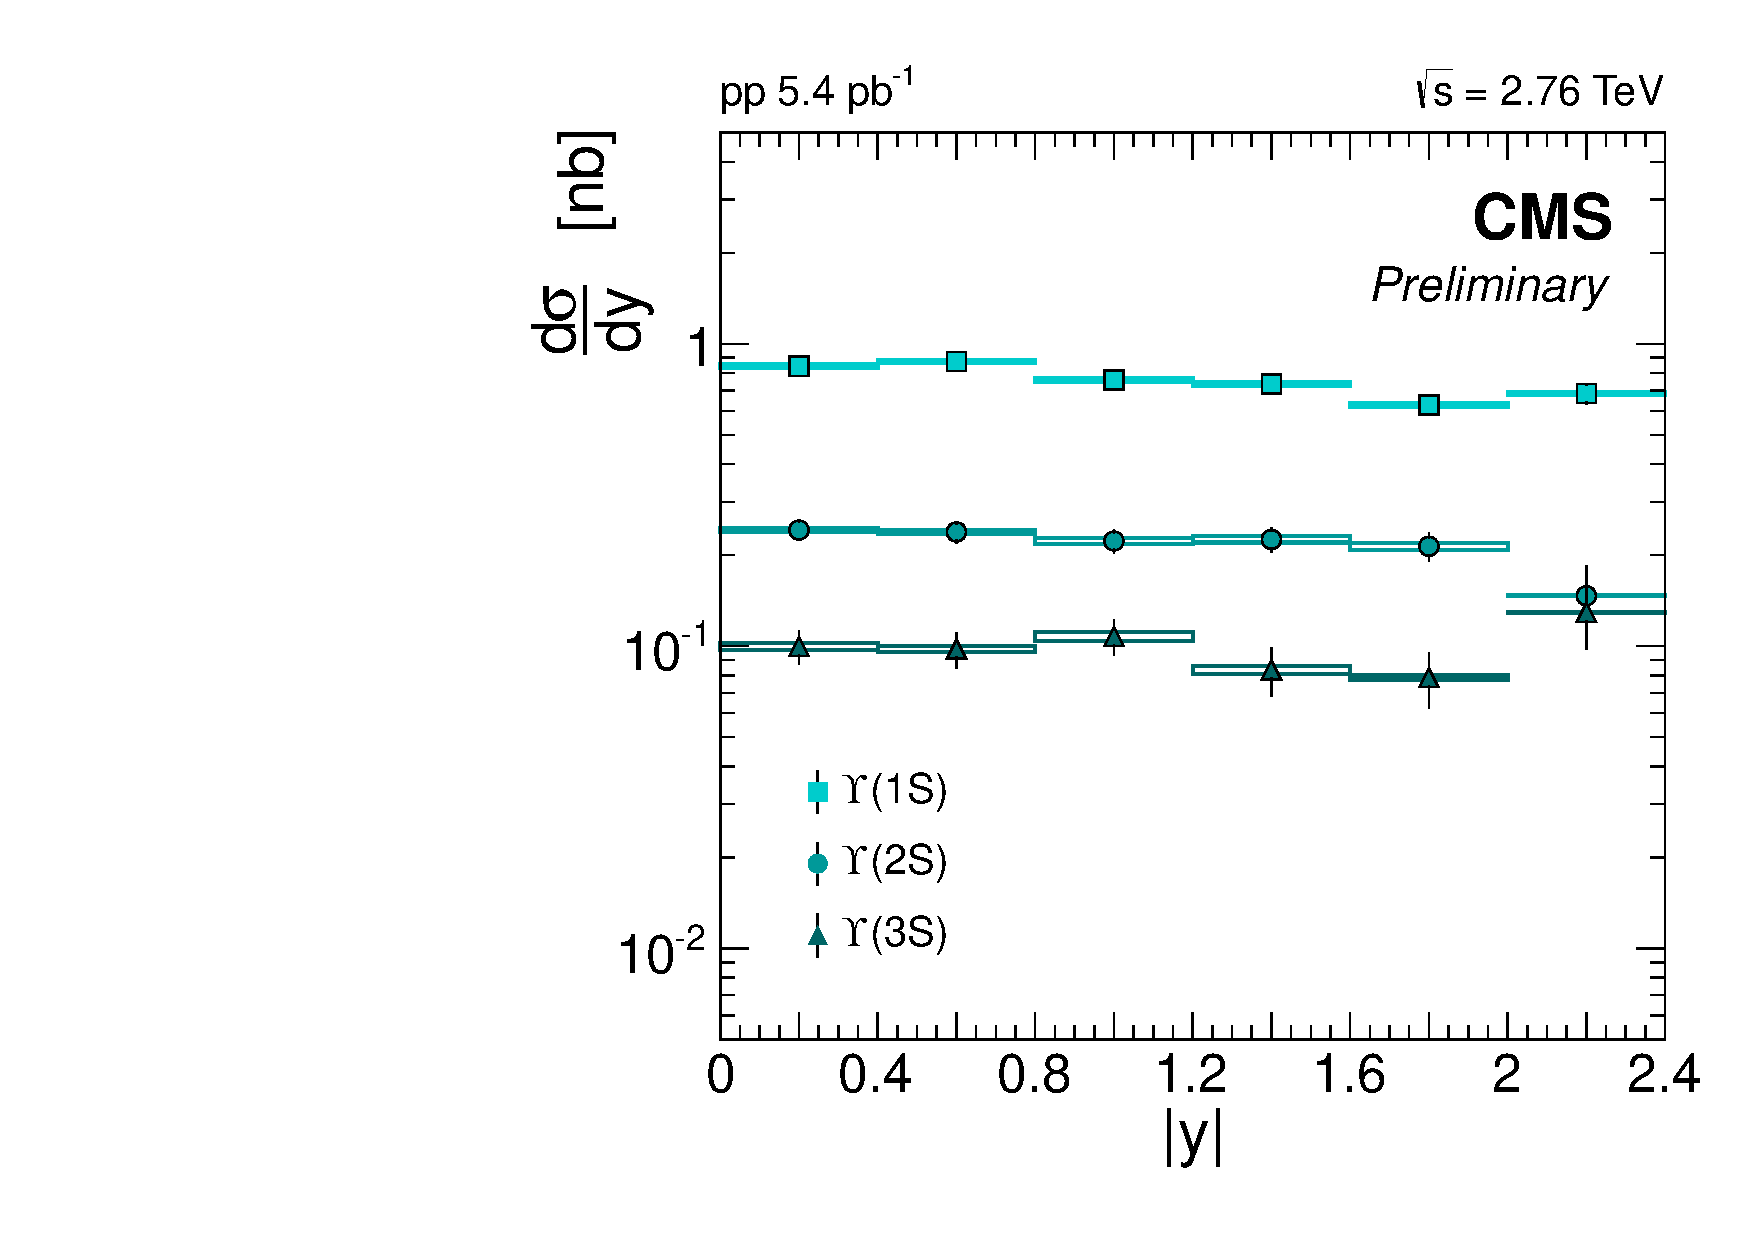
\includegraphics[width=0.7\textwidth]{Results/CS1S_ppRap.pdf}
  \caption{\PgUa, \PgUb, \PgUc\ production cross section in pp
  collisions as a function of $\pt$.}
  \label{fig:CSpprap} 
\end{centering}
\end{figure}
%

\begin{table}[htp]
\begin{centering}
\begin{tabular}{|c|c|c|c|}                                      
\hline
pp %, p$^{\mu\mu}_{T} > $0 GeV/c 
&  \multicolumn{3}{c}{$\frac{d\sigma_{nS}}{dy}\cdot B_{\mu\mu}$ [nb]} \vline\\
\hline
%State
 &  $\PgUa$ & $\PgUb$ &  $\PgU$(3S) \\  
 $|y| <$ 0.4        & 0.881 $\pm$ 0.0306 $\pm$ 0.0123  & 0.242 $\pm$ 0.0191 $\pm$ 0.00375  &  0.0998 $\pm$ 0.0126 $\pm$ 0.00255  \\
 0.4 $< |y| <$ 0.8  & 0.91 $\pm$ 0.032 $\pm$ 0.0122    & 0.239 $\pm$ 0.0194 $\pm$ 0.00397  &  0.0978 $\pm$ 0.0132 $\pm$ 0.00235  \\
 0.8 $< |y| <$ 1.2  & 0.789 $\pm$ 0.0307 $\pm$ 0.0124  & 0.223 $\pm$ 0.0201 $\pm$ 0.00539  &  0.108 $\pm$ 0.0144 $\pm$ 0.00386    \\
 1.2 $< |y| <$ 1.6  & 0.762 $\pm$ 0.0319 $\pm$ 0.0117  & 0.225 $\pm$ 0.0218 $\pm$ 0.00523  &  0.0834 $\pm$ 0.0152 $\pm$ 0.00265   \\
 1.6 $< |y| <$ 2    & 0.644 $\pm$ 0.0336 $\pm$ 0.00977 & 0.214 $\pm$ 0.0236 $\pm$ 0.00606  &  0.0786 $\pm$ 0.0164 $\pm$ 0.00129   \\
 2 $< |y| <$ 2.4    & 0.71 $\pm$ 0.0562 $\pm$ 0.0055   & 0.147 $\pm$ 0.0383 $\pm$ 0.000584 &  0.129 $\pm$ 0.0317 $\pm$ 0.000575  \\
\hline

\end{tabular}
\caption{$y$-differential cross section in pp collisions. Listed
uncertainties are statistical (first) and systematic (second).}  
\label{tab:CSppraptab}
\end{centering}
\end{table}

\vfill\newpage
\subsection{Inclusive differential invariant yields in PbPb}
% and
%\texorpdfstring{\RAA}{RAA} of \texorpdfstring{$\PgU$}{Y}(1S,2S)  in PbPb}
\label{subsec:csaa}

The  differential \PgU\ invariant yield %cross section
 in PbPb collisions, normalized 
% by the thickness function \TAA, and 
 by the number of minimum bias events, \NMB,
 is
computed as a function of $\pt$ and $y$,
%computed via the following Equations \ref{eq:nypt} and \ref{eq:nyrap}
%for $\pt$ and $y$ dependence, respectively:
\begin{eqnarray} 
\label{eq:nypt}
\YPbPb(\pt) \equiv \dfrac{1}{\TAA} \cdot \dfrac{1}{\Delta y} \dfrac{\text{d}N\left( AA\rightarrow
 \PgU(nS)X\right)}{\text{d}\pt} \cdot B_{\mu\mu} &=&
 \dfrac{1}{\TAA}
 \dfrac{1}{\NMB}\cdot\dfrac{\NFitnSPbPb}{\alpha\ \varepsilon_{\rm PbPb}\
 \Delta \pt\Delta y} \\
\label{eq:nyrap}
\YPbPb(y) \equiv  \dfrac{1}{\TAA} \cdot \dfrac{\text{d}N\left( AA\rightarrow
 \PgU(nS)X\right)}{\text{d}y} \cdot B_{\mu\mu} &=&
 \dfrac{1}{\TAA} 
  \dfrac{1}{\NMB} \cdot \dfrac{\NFitnSPbPb}{\alpha\ \varepsilon_{\rm PbPb}\ \Delta y} 
 \end{eqnarray}    
% 
where
\begin{itemize}
\item{\NFitnSPbPb\ is the number of measured $\PgU$ decaying to
two muons, from the fit
to data;}
\item{$\alpha$ is the geometric acceptance, as computed in Section
\ref{sec:Efficiency};}
\item{$\varepsilon_{\rm PbPb}$ is the dimuon trigger and reconstruction
efficiency computed from the embedded sample;}
\item{\NMB = 1.161$\times 10^{9}$ is the number of minimum bias
PbPb events, after correction for a minimum bias selection efficiency
of 97\%;}
%\item{\TAA\ is the expected value of the nuclear overlap function,
%obtained from a Glauber model calculation; XXX REF XXX}
\item{$\Delta y$ and $\Delta \pt$ are the bin widths in rapidity and
$\pt$, respectively.}
\end{itemize}

The  $\PgUa$ and $\PgUb$  yields, \YPbPb, are compared as a function of $\pt$  and as function of $y$ in Figure \ref{fig:CSaapt1vs2}.%in Figure \ref{fig:CSaarap1vs2}.
% XXX MORE LATER XXX

In order to compare the PbPb yields to the pp cross section, the
invariant corrected yields in PbPb collisions are divided by the
nuclear thickness
function \TAA, which is obtained from a Glauber model calculation,
\ie, $\YPbPb/\TAA$. These $\PgUa$ normalized yields in PbPb collisions
are compared to the pp cross section as a function of $\pt$  and as function of $y$
in Figure \ref{fig:CSaapt}.% in Figure~\ref{fig:CSaarap}.
 Tabulated versions of the invariant yields
are reported in Section~\ref{subsec:raa}, alongside with the tabulated
\RAA results.
\vfill\newpage

\begin{figure}[ht]
\begin{centering}  
  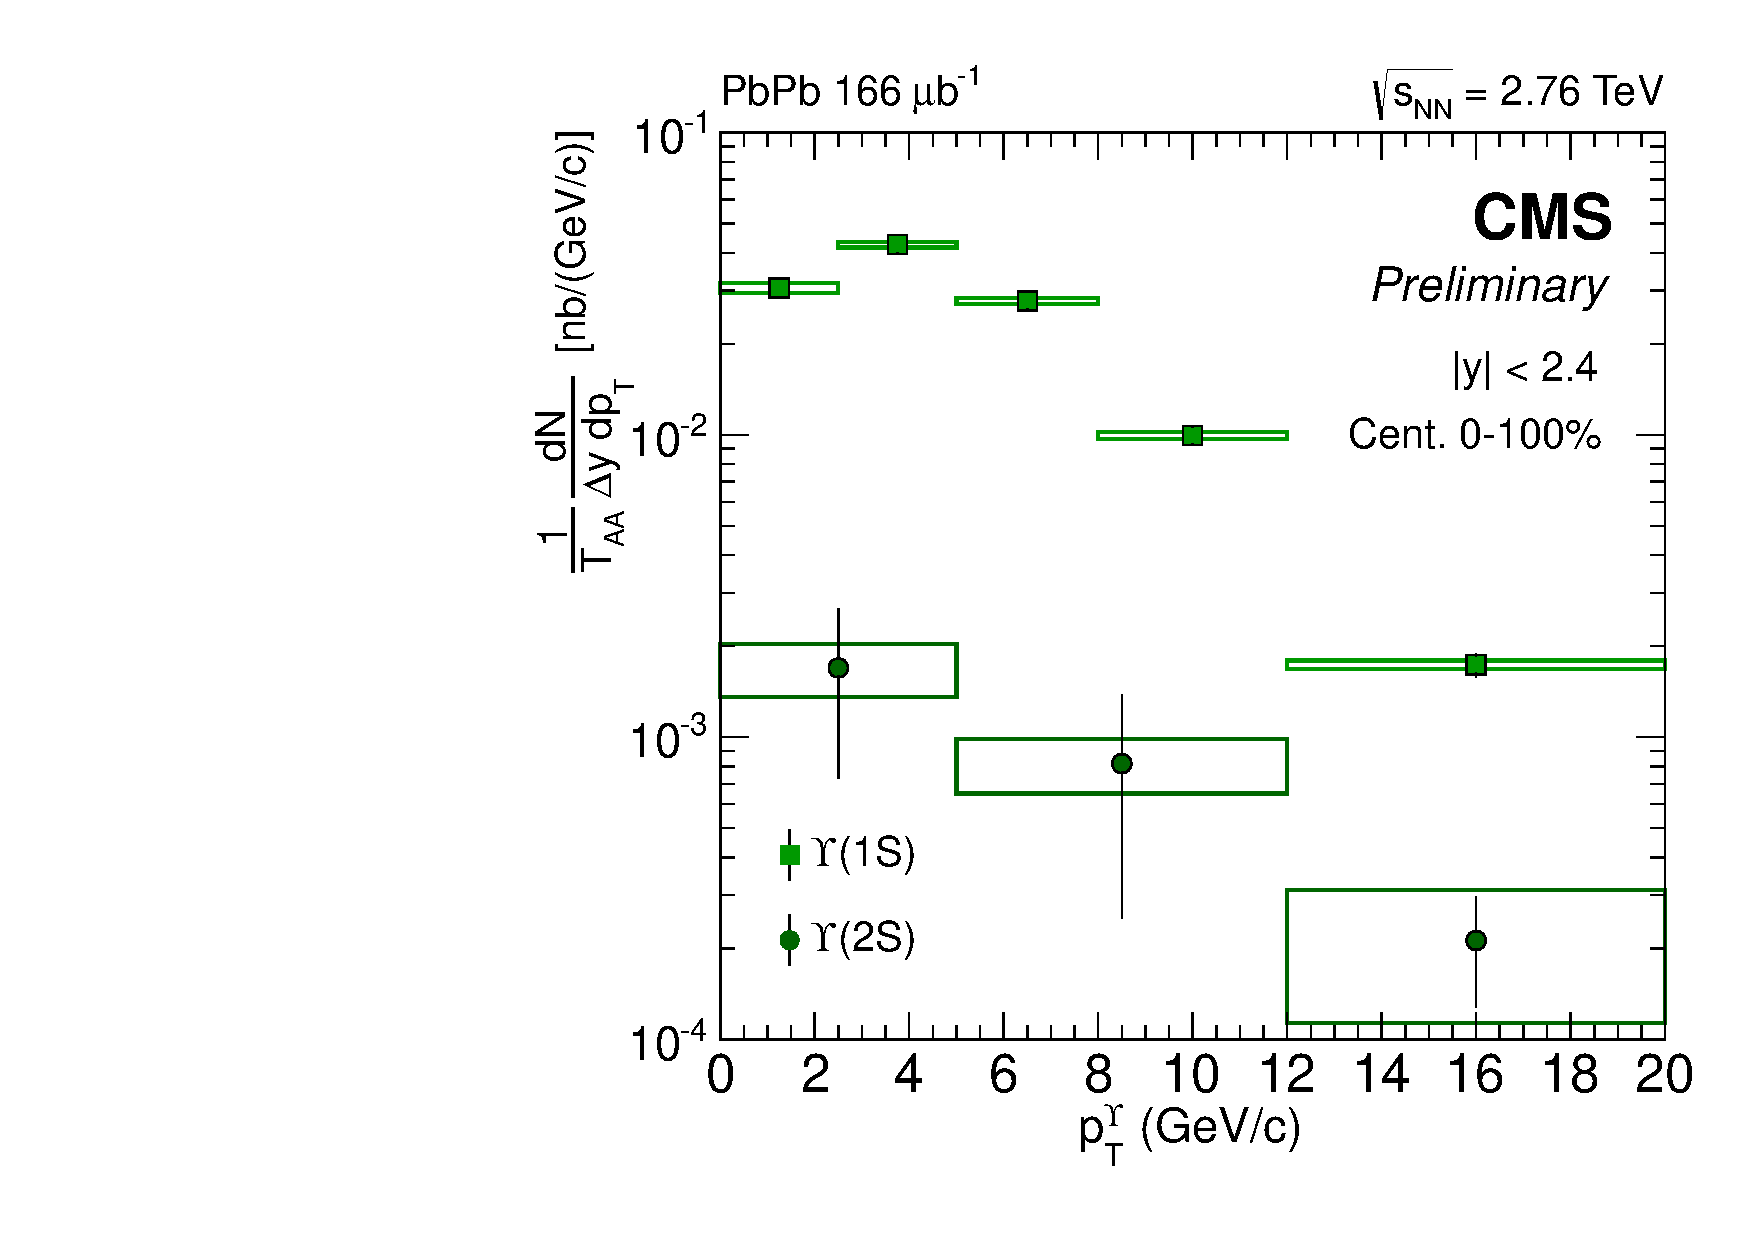
\includegraphics[width=0.49\textwidth]{Results/CS_AAPt.pdf}
  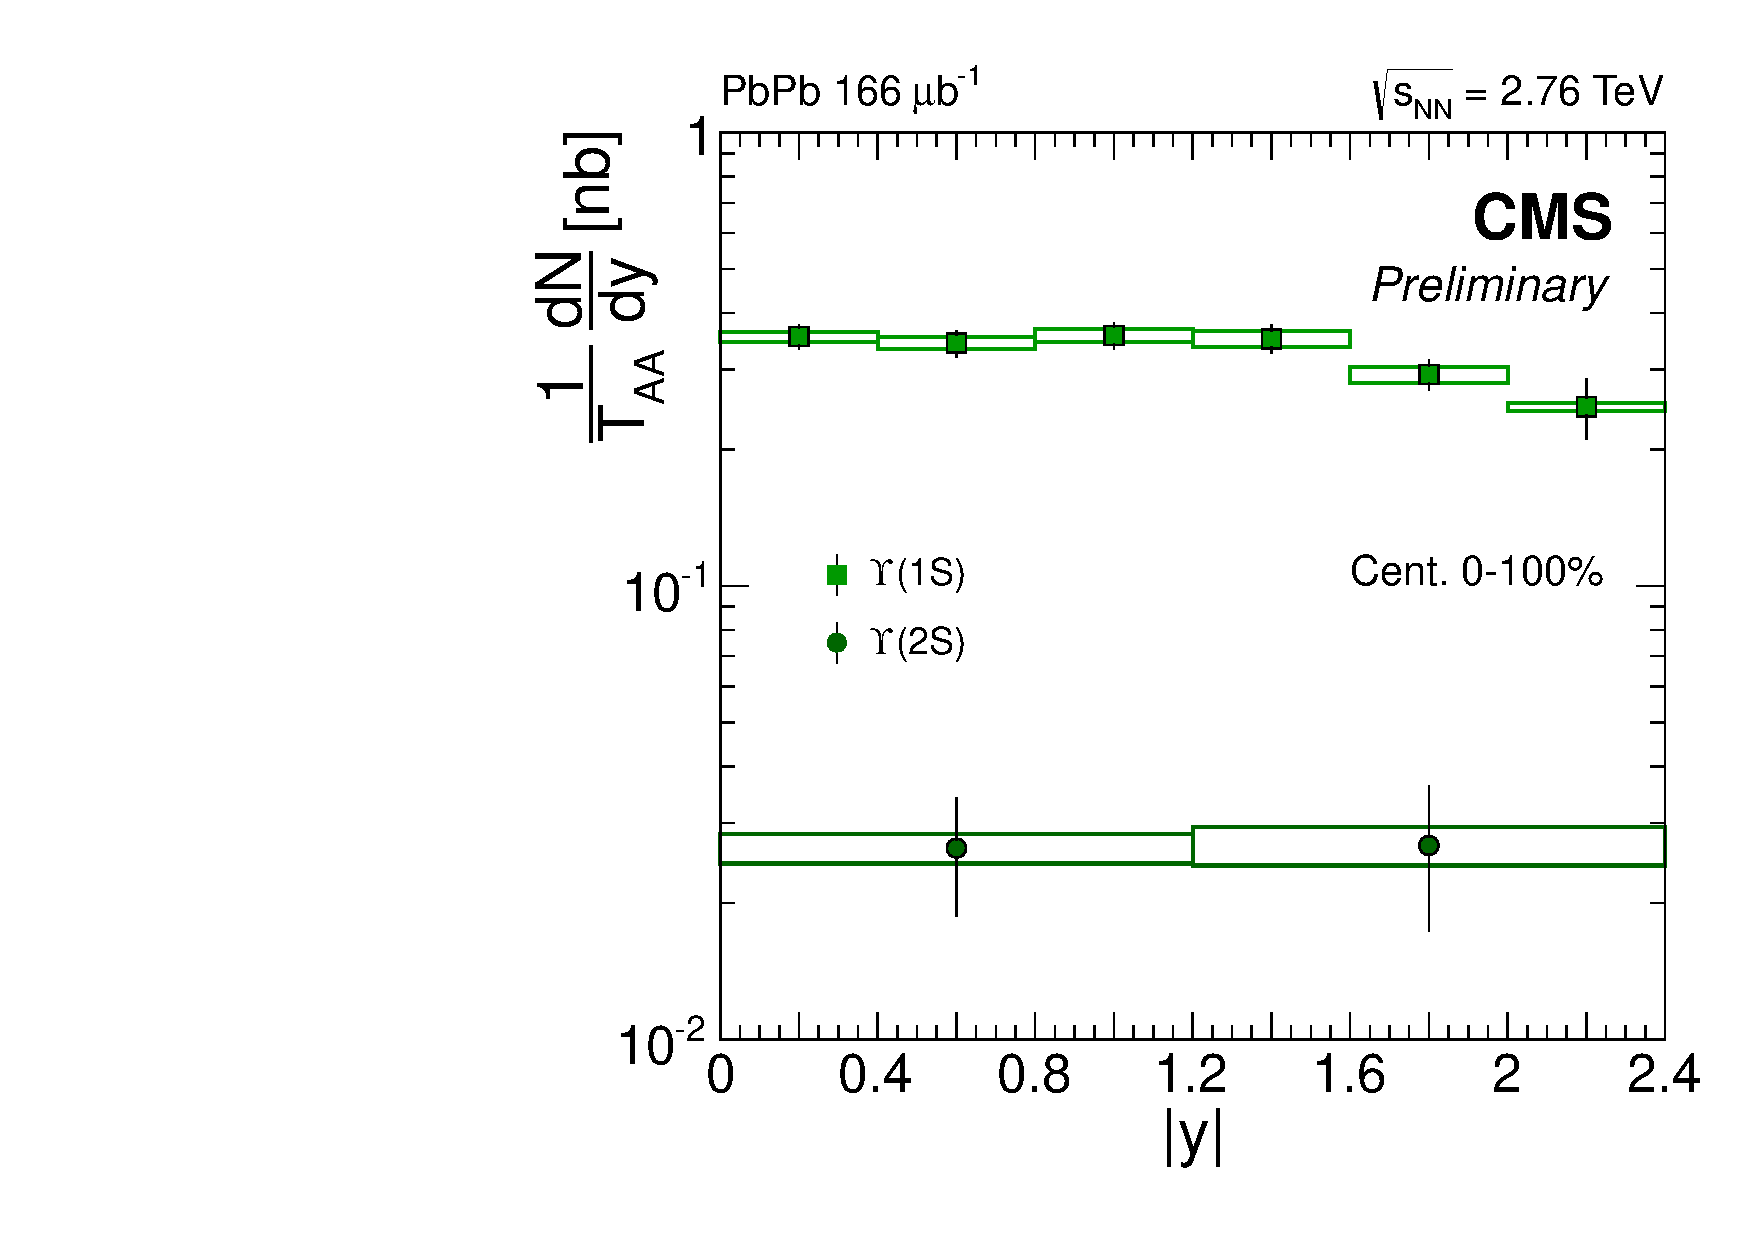
\includegraphics[width=0.49\textwidth]{Results/CS_AA_Rap.pdf}
  \caption{Invariant yields of \PgUa and \PgUb\ in PbPb collisions as
    a function of $\pt$ (left) and $|y|$ (right).}
  \label{fig:CSaapt1vs2} 
\end{centering}  
\end{figure}


\begin{figure}[thp]
\begin{centering}  
  \includegraphics[width=0.49\textwidth]{Results/CS1S_ppAAPt.pdf}
  \includegraphics[width=0.49\textwidth]{Results/CS1S_ppAA_Rap.pdf}
 \caption{$\PgUa$ production cross section in pp collisions and
   normalized invariant yields $\YPbPb/\TAA$ in PbPb collisions as a
   function of $\pt$ (left), and  as a function of $y$ (right).}
  \label{fig:CSaapt} 
\end{centering}  
\end{figure}




\subsection{Nuclear modification factor \RAA}
% and
%\texorpdfstring{\RAA}{RAA} of \texorpdfstring{$\PgU$}{Y}(1S,2S)  in PbPb}
\label{subsec:raa}

This formulation allows for the direct comparison of the pp cross section with
the invariant yield measured in PbPb (divided by \TAA). From the pp cross section and the PbPb yield, the nuclear
modification factor
\begin{equation} \label{eq:raa2}
\RAA = \dfrac{\mathcal{L}_{pp}}{\TAA\NMB}\cdot\dfrac{\text{N}^{\PgU}_{\text{PbPb}}}{\text{N}^{\PgU}_{pp}} \cdot \dfrac{\varepsilon_{\rm pp}}{\varepsilon_{\rm PbPb}} 
 \end{equation}  
 can be determined, as a function of $\pt$ and $y$, in order to estimate the suppression in PbPb collisions.
 
The nuclear suppression factor \RAA\ of $\PgUa$ and $\PgUb$ is plotted respectively as a function of $\pt$ and $y$ in Figure~\ref{fig:raapt} and Figure~\ref{fig:raarap}.

The PbPb yields, \YPbPb, and \RAA\ for $\PgUa$ and $\PgUb$ are displayed as a function of $\pt$ and $y$ in Tables~\ref{tab:CSaapttab} and \ref{tab:CSaaraptab}, respectively.

\begin{figure}[h]
\begin{centering}       
  \includegraphics[width=0.75\textwidth]{Results/RAA_Pt.pdf}
  \caption{Nuclear modification factor \RAA\ for \PgUa\ and \PgUb\ 
  as a function of $\pt$.}
  \label{fig:raapt} 
\end{centering}
\end{figure}

\begin{table}[hbtp]
\begin{centering}
\begin{tabular}{|c|c|c|}                                      
\hline
%$|y| < $2.4 & $\frac{d\sigma_{1S}}{dyd\pt}\cdot B_{\mu\mu}$[nb
%c/GeV] & \RAA[\PgUa] \vline \\
$|y| < $2.4 & $\YPbPb[\PgUa]/\TAA$ [nb] & \RAA[\PgUa]  \\
\hline
\pt [{\rm GeV}/c] $<$ 2.5       & 0.0306 $\pm$ 0.00176 $\pm$ 0.0011    & 0.42 $\pm$ 0.028 $\pm$ 0.0636  \\
2.5 $<$ \pt [{\rm GeV}/c] $<$ 5 & 0.0426 $\pm$ 0.00264 $\pm$ 0.000815  & 0.404 $\pm$ 0.0283 $\pm$ 0.0508\\
5 $<$ \pt [{\rm GeV}/c] $<$ 8   & 0.0277 $\pm$ 0.00186 $\pm$ 0.000797  & 0.444 $\pm$ 0.0333 $\pm$ 0.0722\\
8 $<$ \pt [{\rm GeV}/c] $<$ 12  & 0.00994 $\pm$ 0.000745 $\pm$ 0.000228& 0.473 $\pm$ 0.0417 $\pm$ 0.051  \\
12 $<$ \pt [{\rm GeV}/c] $<$ 20 & 0.00174 $\pm$ 0.000162 $\pm$ 5.4e-05 & 0.429 $\pm$ 0.0477 $\pm$ 0.0432\\

\hline
$|y| < $2.4 & $\YPbPb[\PgUb]/\TAA$ [nb] & \RAA[\PgUb]  \\
\hline
\pt [{\rm GeV}/c] $<$ 5          & 0.00169 $\pm$ 0.00096 $\pm$0.00033 & 0.0821$\pm$ 0.0471 $\pm$ 0.0182 \\  
5 $<$ \pt [{\rm GeV}/c] $<$ 12   & 0.00082 $\pm$ 0.00056 $\pm$0.00016 & 0.0656$\pm$ 0.0457 $\pm$ 0.0115 \\  
12 $<$ \pt [{\rm GeV}/c] $<$ 20  & 0.00021 $\pm$ 8.5e-05 $\pm$9.9e-05 & 0.141$\pm$ 0.0585 $\pm$ 0.025 \\  
\hline

% \pt [{\rm GeV}/c] $<$ 6.5        & 0.025 $\pm$ 0.0015 $\pm$
% 0.00063    %%% THAT'S PP in large bins.
% 6.5 $<$ \pt [{\rm GeV}/c] $<$ 10 & 0.0066 $\pm$ 0.00056 $\pm$ 0.00048 
% 10 $<$ \pt [{\rm GeV}/c] $<$ 20  & 0.0026 $\pm$ 0.00025 $\pm$
% 0.00012 

\end{tabular}
\caption{Normalized yields $\YPbPb/\TAA$ and \RAA\ as a function of $\pt$ for \PgUa\ (top) and \PgUb\ (bottom) states. Listed
uncertainties are statistical (first) and systematic (second).}  
\label{tab:CSaapttab}
\end{centering}
\end{table}


\begin{figure}[h]
\begin{centering}       
  \includegraphics[width=0.75\textwidth]{Results/RAA_Rap.pdf}
  \caption{Nuclear modification factor \RAA\ for \PgUa\ and \PgUb\ 
  as a function of rapidity.}
  \label{fig:raarap} 
\end{centering}
\end{figure}

% pt [{\rm GeV}/c] $<$ 2.5 0.033 0.016 0.048 0.11 0.11 0.16 0.18
% 2.5 $<$ pt [{\rm GeV}/c] $<$ 5 0.032 0.0068 0.032 0.1 0.098 0.15 0.17
% 5 $<$ pt [{\rm GeV}/c] $<$ 8 0.029 0.0054 0.058 0.077 0.077 0.13 0.15
% 8 $<$ pt [{\rm GeV}/c] $<$ 12 0.046 0.012 0.012 0.057 0.056 0.094 0.13
% 12 $<$ pt [{\rm GeV}/c] $<$ 20 0.06 0.0025 0.0064 0.037 0.038 0.08 0.12
\begin{table}[hbtp]
\begin{centering}
\begin{tabular}{|c|c|c|c|}                                      
\hline
%p$^{\mu\mu}_{T} > $0 GeV/c & $\frac{d\sigma_{1S}}{dy}\cdot B_{\mu\mu}$
%[nb] & \RAA[\PgUa]  \vline \\
%p$^{\mu\mu}_{T} > $0 GeV/c 
& $\YPbPb[\PgUa]/\TAA$ [nb] & \RAA[\PgUa]  \\
\hline
$|y| <$ 0.4        & 0.355$\pm$ 0.022$\pm$  0.0078 & 0.402$\pm$0.025$\pm$ 0.404\\  
0.4 $< |y| <$ 0.8  & 0.343$\pm$ 0.023$\pm$  0.0121 & 0.377$\pm$0.025$\pm$ 0.38 \\  
0.8 $< |y| <$ 1.2  & 0.357$\pm$ 0.024$\pm$  0.0198 & 0.452$\pm$0.030$\pm$ 0.46\\  
1.2 $< |y| <$ 1.6  & 0.352$\pm$ 0.025$\pm$  0.0134 & 0.461$\pm$0.034$\pm$ 0.466\\  
1.6 $< |y| <$ 2    & 0.3  $\pm$ 0.025$\pm$  0.0192 & 0.466$\pm$0.039$\pm$ 0.484\\  
2 $< |y| <$ 2.4    & 0.249$\pm$ 0.037$\pm$  0.0077 & 0.35 $\pm$0.053$\pm$ 0.373x \\  
\hline   


\hline
%p$^{\mu\mu}_{T} < $0 GeV/c & $\frac{d\sigma_{2S}}{dy}\cdot B_{\mu\mu}$
%[nb] & \RAA[\PgUb] \vline \\
%p$^{\mu\mu}_{T} < $0 GeV/c 
& $\YPbPb[\PgUb]/\TAA$ [nb] & \RAA[\PgUb]  \\
\hline
$|y| <$ 1.2       & 0.0264 $\pm$0.0077 $\pm$ 0.0019 & 0.113 $\pm$ 0.033 $\pm$ 0.034 \\  
1.2 $< |y| <$ 2.4 & 0.0268 $\pm$0.0095$\pm$  0.0025 & 0.135 $\pm$ 0.048 $\pm$ 0.073  \\  
\hline

\end{tabular}
\caption{Normalized yields $\YPbPb/\TAA$ and \RAA\ as a function of $y$ for \PgUa (top) and \PgUb\ (bottom) states. Listed
uncertainties are statistical (first) and systematic (second).} 
\label{tab:CSaaraptab} 
\end{centering}
\end{table}

\vfill\newpage
\subsection{Centrality dependence of \texorpdfstring{$\PgU$}{Y}(1S) and \texorpdfstring{$\PgU$}{Y}(2S) suppression in PbPb collisions}
\label{subsec:raah}
The centrality dependence of the suppression has been computed
in various \Npart\ bins for \PgUa\ and \PgUb. Some additional
features should be noted with respect to the previous (Ref. here:
HIN-11-011) analysis:
\begin{itemize}
\item{The 1S analysis is now performed with the yield extraction
method using the loose single muon $\pt$ cut defined in Section
\ref{sec:Yields};}
\item{An additional peripheral bin in the 1S result is displayed: The
peripheral 50-100 bin is now splitted into 50-70 and 70-100 percent.}
\item{The pp sample used herein results of a much longer data taking
period than previously, reducing significantly the uncertainty on the
suppression. The Y analysis in pPb (Ref. here: HIN-13-003) has
estimated the normalisation ratio between 2011 and 2013 pp cross
sections to be (1.6 $\pm$ 0.4), resulting in a difference not greater
than 1.5 standard deviations.}
\end{itemize}

Table \ref{tab:centraa} reports the invariant yield divided by
\TAA\ in centrality classes for 1S and 2S in upper and lower
panels, respectively. Figure \ref{fig:raacompcent} shows the
corresponding \RAA\ measured in this analysis (1S in orange, 2S in
blue) compared with the previous measurement (1S in green, 2S in white
circles.)


\begin{figure}[h]
\begin{centering}       
  \includegraphics[width=0.8\textwidth]{Results/RAA_nPart_4bins.pdf}
  \caption{Nuclear modification factor \RAA\ for \PgUa\ and \PgUb\ 
  as a function of the number of participants, \Npart.}
  \label{fig:raacompcent} 
\end{centering}
\end{figure}

\begin{table}[hbtp]
  \begin{centering}
    \begin{tabular}{|c|c|c|}
      \hline
%      Centrality percentiles & 1/\TAA.invariant yield & \RAA\ \\                                               
      Centrality percentiles & $\YPbPb[\PgUa]/\TAA$ [nb] &  \RAA[\PgUa]\ \\                                               
      \hline
%      \pt^{\mu} <$ 3.5 or 4 GeV &  $\frac{dN_{1S}}{\TAA\cdot
%      dy}\cdot B_{\mu\mu}$
%[nb] & \RAA[\PgUa] \\
%      \hline 
      0-5    &1.12 $\pm$ 0.0998 $\pm$ 0.0431  &  0.31 $\pm$ 0.0276 $\pm$ 0.0508   \\  
      5-10   &1.38 $\pm$ 0.112 $\pm$ 0.0486   &  0.383 $\pm$ 0.0311 $\pm$ 0.0557  \\  
      10-20  &1.5 $\pm$ 0.0943 $\pm$ 0.0488   &  0.415 $\pm$ 0.0261 $\pm$ 0.0554  \\  
      20-30  &1.62 $\pm$ 0.12 $\pm$ 0.0508    &  0.447 $\pm$ 0.0331 $\pm$ 0.057   \\  
      30-40  &1.85 $\pm$ 0.161 $\pm$ 0.0752   &  0.513 $\pm$ 0.0445 $\pm$ 0.0827   \\  
      40-50  &2.05 $\pm$ 0.222 $\pm$ 0.106    &  0.567 $\pm$ 0.0613 $\pm$ 0.115   \\  
      50-70  &2.76 $\pm$ 0.281 $\pm$ 0.12     &  0.764 $\pm$ 0.0778 $\pm$ 0.13    \\  
      70-100 &4.15 $\pm$ 0.746 $\pm$ 0.292    & 1.15 $\pm$ 0.207 $\pm$ 0.314     \\  
      0-100  &1.537 $\pm$ 0.081 $\pm$ 0.028   & 0.425 $\pm$ 0.024$\pm$ 0.034 \\   
      \hline 
      pp     &3.613$\pm$ 0.066 $\pm$ 0.032 & --- \\
      \hline  
      \hline          
%      \pt^{\mu} <$ 4 GeV &  $\frac{d\sigma_{2S}}{\TAA\cdot dy}\cdot B_{\mu\mu}$
%[nb] & \RAA[\PgUb]   \\
%      \pt^{\mu} <$ 4 GeV 
      &  $\YPbPb[\PgUb]/\TAA$ [nb] 
%      $\frac{d\sigma_{2S}}{\TAA\cdot dy}\cdot B_{\mu\mu}$
%[nb] 
& \RAA[\PgUb]   \\
     \hline
      0-10   & 0.076 $\pm$ 0.045 $\pm$0.039  & 0.074 $\pm$ 0.044 $\pm$ 0.038 \\  
      10-30  & 0.092 $\pm$ 0.044 $\pm$0.056  & 0.090 $\pm$ 0.042 $\pm$ 0.054  \\  
      30-50  & 0.293 $\pm$ 0.079 $\pm$0.103  & 0.286 $\pm$ 0.077 $\pm$ 0.100   \\  
      50-100 & 0.226 $\pm$ 0.149 $\pm$0.116  & 0.220 $\pm$ 0.145 $\pm$ 0.113   \\  
      0-100  & 0.119 $\pm$ 0.029 $\pm$ 0.002 &0.116 $\pm$ 0.028  $\pm$ 0.013  \\  
      \hline 
      pp     &1.026 $\pm$ 0.042 $\pm$ 0.016 & --- \\
      \hline 

% total_sigma(3S)_pp = 0.128601 $\pm$ 0.010113
% total_sigma(3S)_AA = 0.00371262 $\pm$ 0.00695088
% Raa_3S = 0.0288693 $\pm$ 0.0540977 stat.
    \end{tabular}
    \caption{Normalized yields $\YPbPb/\TAA$ and nuclear suppression factor $\RAA$ for different
      centrality bins (and for centrality-integrated) for \PgUa\ and \PgUb.}
    \label{tab:centraa}
  \end{centering}
\end{table}

\subsection{Systematic uncertainties}
A break-down of the systematic uncertainties is given in the following
Table \ref{tab:breakdown} for the kinematic dependency analysis of
1S. The listed uncertainties from left to right
are:
\begin{itemize}
\item[-] Statistical uncertainty from the nominal fit to the
      pp yield,
\item[-] Systematic uncertainty from fit variations on pp,
\item[-] Systematic uncertainty from fit variations on PbPb,
\item[-] Scale factor uncertainty for efficiency correction, from tag-and-probe in
  pp,
\item[-] Scale factor uncertainty for efficiency correction, from tag-and-probe in
  AA
\item[-] Total of 'correlated' point-to-point
  systematic uncertainties, computed as the quadratic sum of the four
  previous columns + the systematic uncertainty due to shape
  variations (quoted 'Sys Err' in the efficiency chapter),
\item[-] Quadratic sum of point-to-point and global uncertainty.
\end{itemize}
\newpage
\begin{landscape}
\begin{table}[p]
  \begin{centering}
      \begin{tabular}{|c|c|c|c|c|c|c|c|c|}
        \hline
        $\pt$ bin & Stat. (pp) & Stat. (AA) & Syst(PDF)$_{pp}$ & Syst(PDF)$_{AA}$ & TNP$_{pp}$ &  TNP$_{AA}$ & Correlated &
        total\\
        \hline
        pt [{\rm GeV}/c] $<$ 2.5 & 0.034 & 0.057 & 0.076 & 0.091 & 0.007 & 0.040 & 0.133 & 0.151      \\
        2.5 $<$ pt [{\rm GeV}/c] $<$ 5 & 0.032 & 0.061 & 0.050 & 0.065 & 0.006 & 0.040 & 0.103 & 0.126\\
        5 $<$ pt [{\rm GeV}/c] $<$ 8 & 0.034 & 0.066 & 0.039 & 0.125 & 0.006 & 0.038 & 0.146 & 0.163  \\
        8 $<$ pt [{\rm GeV}/c] $<$ 12 & 0.046 & 0.074 & 0.023 & 0.043 & 0.006 & 0.035 & 0.081 & 0.108 \\
        12 $<$ pt [{\rm GeV}/c] $<$ 20 & 0.060 & 0.093 & 0.008 & 0.038 & 0.007 & 0.034 & 0.071 & 0.101\\
        \hline
        \hline
        $|y| <$ 0.4 & 0.035 & 0.064 &  0.030 & 0.055 & 0.004 & 0.010 &        0.063 & 0.005 \\
        0.4 $< |y| <$ 0.8   & 0.035 & 0.068 &  0.026 & 0.110 & 0.004 & 0.011 & 0.114 & 0.009\\
        0.8 $< |y| <$ 1.2  & 0.039 & 0.068 &  0.038 & 0.175 & 0.004 & 0.018 & 0.180 & 0.019 \\
        1.2 $< |y| <$ 1.6  & 0.042 & 0.074 &  0.039 & 0.093 & 0.007 & 0.053 & 0.114 & 0.010 \\
        1.6 $< |y| <$ 2    & 0.052 & 0.085 &  0.051 & 0.216 & 0.012 & 0.108 & 0.247 & 0.038 \\
        2 $< |y| <$ 2.4    & 0.079 & 0.151 &  0.082 & 0.281 & 0.015 & 0.150 & 0.329 & 0.066\\
      \end{tabular}
      \caption{Systematic uncertainties recap for $\PgUa$, in
        ($\pt$,y)-differential  R$_{AA}$ analyses. }  
      \label{tab:breakdown}
    \end{centering}
\end{table}
\end{landscape}

Table \ref{tab:breakdownPart} sums up the systematic uncertainties
used in the centrality dependence result.
\begin{itemize}
\item[-] Systematic uncertainty from fit variations on PbPb,
\item[-] Scale factor for efficiency correction, from tag-and-probe in
  pp,
\item[-] Uncertainty on the value of the nuclear thickness function
\item[-] Global pp uncertainty: summing up luminosity, integrated
  scale factor for pp efficiency, statistical and systematic
  uncertainty from fitting,
\item[-] Total of 'correlated' point-to-point
  systematic uncertainties, computed as the quadratic sum of the four
  previous columns
\item[-] Total of 'correlated' and global uncertainty.
\end{itemize}
\begin{table}[hbtp]
  \begin{centering}
    \begin{tabular}{|c|c|c|c|c|c|c|}
      \hline
      1S Centrality & Syst(PDF)$_{AA}$ & TNP$_{AA}$ & T$_{AA}$ &
      Global pp & Correlated & total\\
      \hline
      0-5   &0.144 &0.036 &0.041 &0.035 &0.160 &0.164 \\
      5-10  &0.120 &0.038 &0.046 &0.035 &0.141 &0.146 \\
      10-20 &0.103 &0.037 &0.052 &0.035 &0.129 &0.134\\
      20-30 &0.085 &0.038 &0.066 &0.035 &0.122 &0.127\\
      30-40 &0.120 &0.038 &0.084 &0.035 &0.157 &0.161\\
      40-50 &0.157 &0.038 &0.109 &0.035 &0.199 &0.202\\
      50-70 &0.054 &0.039 &0.147 &0.035 &0.167 &0.171\\
      70-100&0.215 &0.039 &0.154 &0.035 &0.271 &0.273\\
      \hline
      2S Centrality & Syst(PDF)$_{AA}$ & TNP$_{AA}$ & T$_{AA}$ &
      Global pp & Correlated & total\\
      \hline
     0-10 &  0.458 &0.035 &0.043 &0.056 &0.510 &0.513 \\
     10-30 & 0.560 &0.036 &0.058 &0.056 &0.603 &0.605 \\
     30-50 & 0.255 &0.036 &0.093 &0.056 &0.346 &0.350 \\
     50-100 &0.440 &0.036 &0.150 &0.056 &0.512 &0.515 \\
      \hline
    \end{tabular}
    \caption{Systematic uncertainties recap for $\PgUa$ and $\PgUb$, in
      bins of number of participants. }  
    \label{tab:breakdownPart}
  \end{centering}
\end{table} 

%\subsection{Yields from fitting}
\vfill\newpage
\subsection{Upper limits on Y(3S) production in PbPb collisions}
\label{sec:Y3S}

Once the signal is extracted from the ML fit,
we employ the Feldman-Cousins (FC) prescription to set a limit at $95\%$ confidence level% ~\cite{MCMC}
.
While the expected limit on the nuclear modification factor is close to a
 non-physical (negative) limit, %(i.e. $\RAA(\PgUc) \leq  0$),
the FC prescription guarantees a physically meaningful result and tells us how to smoothly
transition from a one-sided limit to a two-sided interval. In other words, this method will return a two-sided interval
in the case of a significant result, and an upper limit in the case of a non-significant result, the transition
between the two cases being smooth and well-defined from a statistical point of view (i.e. with
a proper coverage).
% %The FC prescription is described in detail in Ref.~\cite{FC}. % Ref missing!
% It uses a likelihood ratio as an ordering principle for selecting the acceptance
%  region and creating confidence bands. The likelihood ratio is defined as the following:
% \begin{equation}
% Q(x)=\frac{P(x|\RAA(\PgUc)_{0})}{P(x|\RAA(\PgUc)_{\text{max}})} \,,
% \end{equation}
% where $Q(x)$ is a likelihood ratio for given $\raa(\PgUc)$, x,  a given $\raa(\PgUc)$ and finally $\raa(\PgUc)_{0}$,
% and $\raa(\PgUc)_{\text{max}}$ is the $\raa(\PgUc)$ for the maximum likelihood among all possible $\raa(\PgUc)$ values.

The Feldman Cousins method is applied via its implementations in
RooStats. In practice the class \verb-HypoTestInverter- is used, with two possible settings: frequentist
(using pseudo-experiments) or asymptotic (using asymptotic formulae). The latter is less reliable and
can only be used as a fast cross-check. The test statistic used is a profile likelihood ratio.

In the lack of MC simulation for the $\PgUc$, we assume the ratio of PbPb to pp efficiencies to be the same for the $\PgUb$ and $\PgUc$, and
take the value (0.95) from the $\PgUb$ simulation.

Systematic uncertainties are included as nuisance parameters in the fit, with a log-normal distribution. The following systematic uncertainties are included for now:

\begin{itemize}
   \item $T_{AA}$ (6.2\%)
   \item pp luminosity (3.7\%)
   \item ratio of efficiencies between pp and PbPb (including the systematic uncertainty on tag and probe) (5.3\%)
   \item number of background events in pp (from the fit variations) (4\%)
   \item number of background events in PbPb (from the fit variations) (2\%)
   \item number of signal events in pp (from the fit variations) (8\%)
   \item number of signal events in PbPb (from the fit variations) (20\%)
\end{itemize}

% This list will be updated soon to match the systematic uncertainties used in the rest of the analysis.

A reliable systematic uncertainty on the $\PgUc$ in PbPb could not be determined from fit variations, given its non significant yield. For this reason,
this systematic uncertainty was deduced in the following way: 
$\textrm{syst} (\PgUa, \textrm{PbPb}) \times \textrm{syst} (\PgUc, \textrm{pp}) / \textrm{syst} (\PgUa, \textrm{pp})$, which gives $0.11 \times 0.08/0.045 = 0.20$.

Using the asymptotic calculation, we obtain an upper limit $\RAA(\PgUc)<0.13$ at 95\% C.L. Using the full frequentist calculation
(using pseudo-experiments), we obtain

\begin{eqnarray*}
 \RAA(\PgUc)<0.14 \text{   at 95\% C.L.}\\ \nonumber
 \RAA(\PgUc)<0.08 \text{   at 68\% C.L.} \nonumber
\end{eqnarray*}


The result of the scan is shown on Fig.~\ref{fig:3SUL}, on the left for the asymptotic calculation and on the right for the frequentist
calculation. Visually, the upper limit is obtained from the place where the 
observed $CL_s$ (red dots) crosses the horizontal threshold (red line, at $0.05 = 1-0.95$ for 95\% C.L.). Fig.~\ref{fig:3SUL_68} shows the scan for the frequentist
calculation, zoomed in on smaller values of $\RAA(\PgUc)$ for the determination of the 68\% C.L. upper limit.


% The confidence interval calculator is tried as well in
% estimating the 95$\%$ confidence interval of the 2S yield, using the asymptotic approach, as a cross-check. 
% The yield extracted of the 2S confidence region at 95\% C.L. is [60,225], with a
% maximum peaking at about 150 candidates, which is compatible with a direct ML fit. Indeed, the latter gives 
% [101,184] at 68\% C.L., or [62,225] at the 95\% C.L.
% 
% The results
% of the frequentist scan for the 3S and of the asymptotic scan for the 2S are reported respectively
% in Figure~\ref{fig:3SUL} and Figure~\ref{fig:2SCI}. 

\begin{figure}[h]
\begin{centering}       
  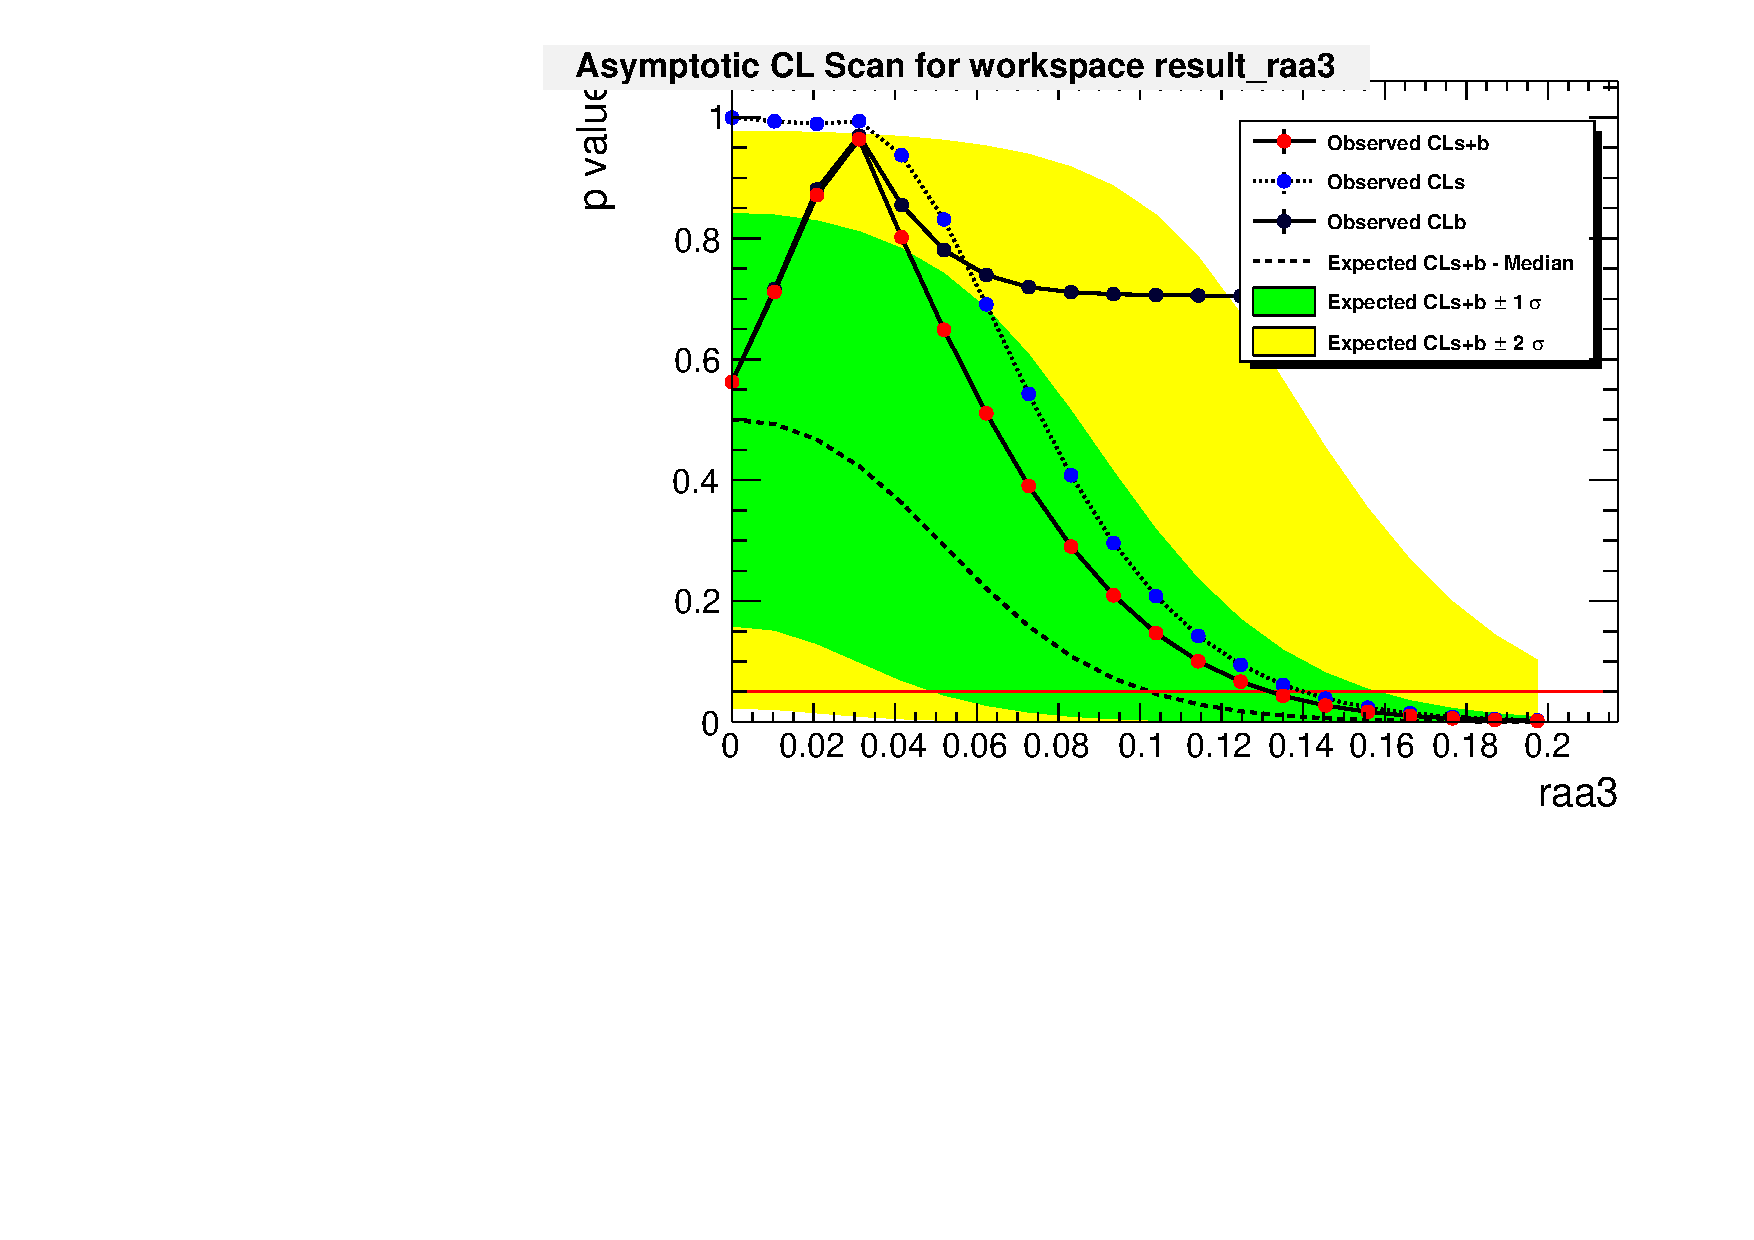
\includegraphics[width=0.49\textwidth]{Results/asymptotic_x3raw_simple.pdf}
  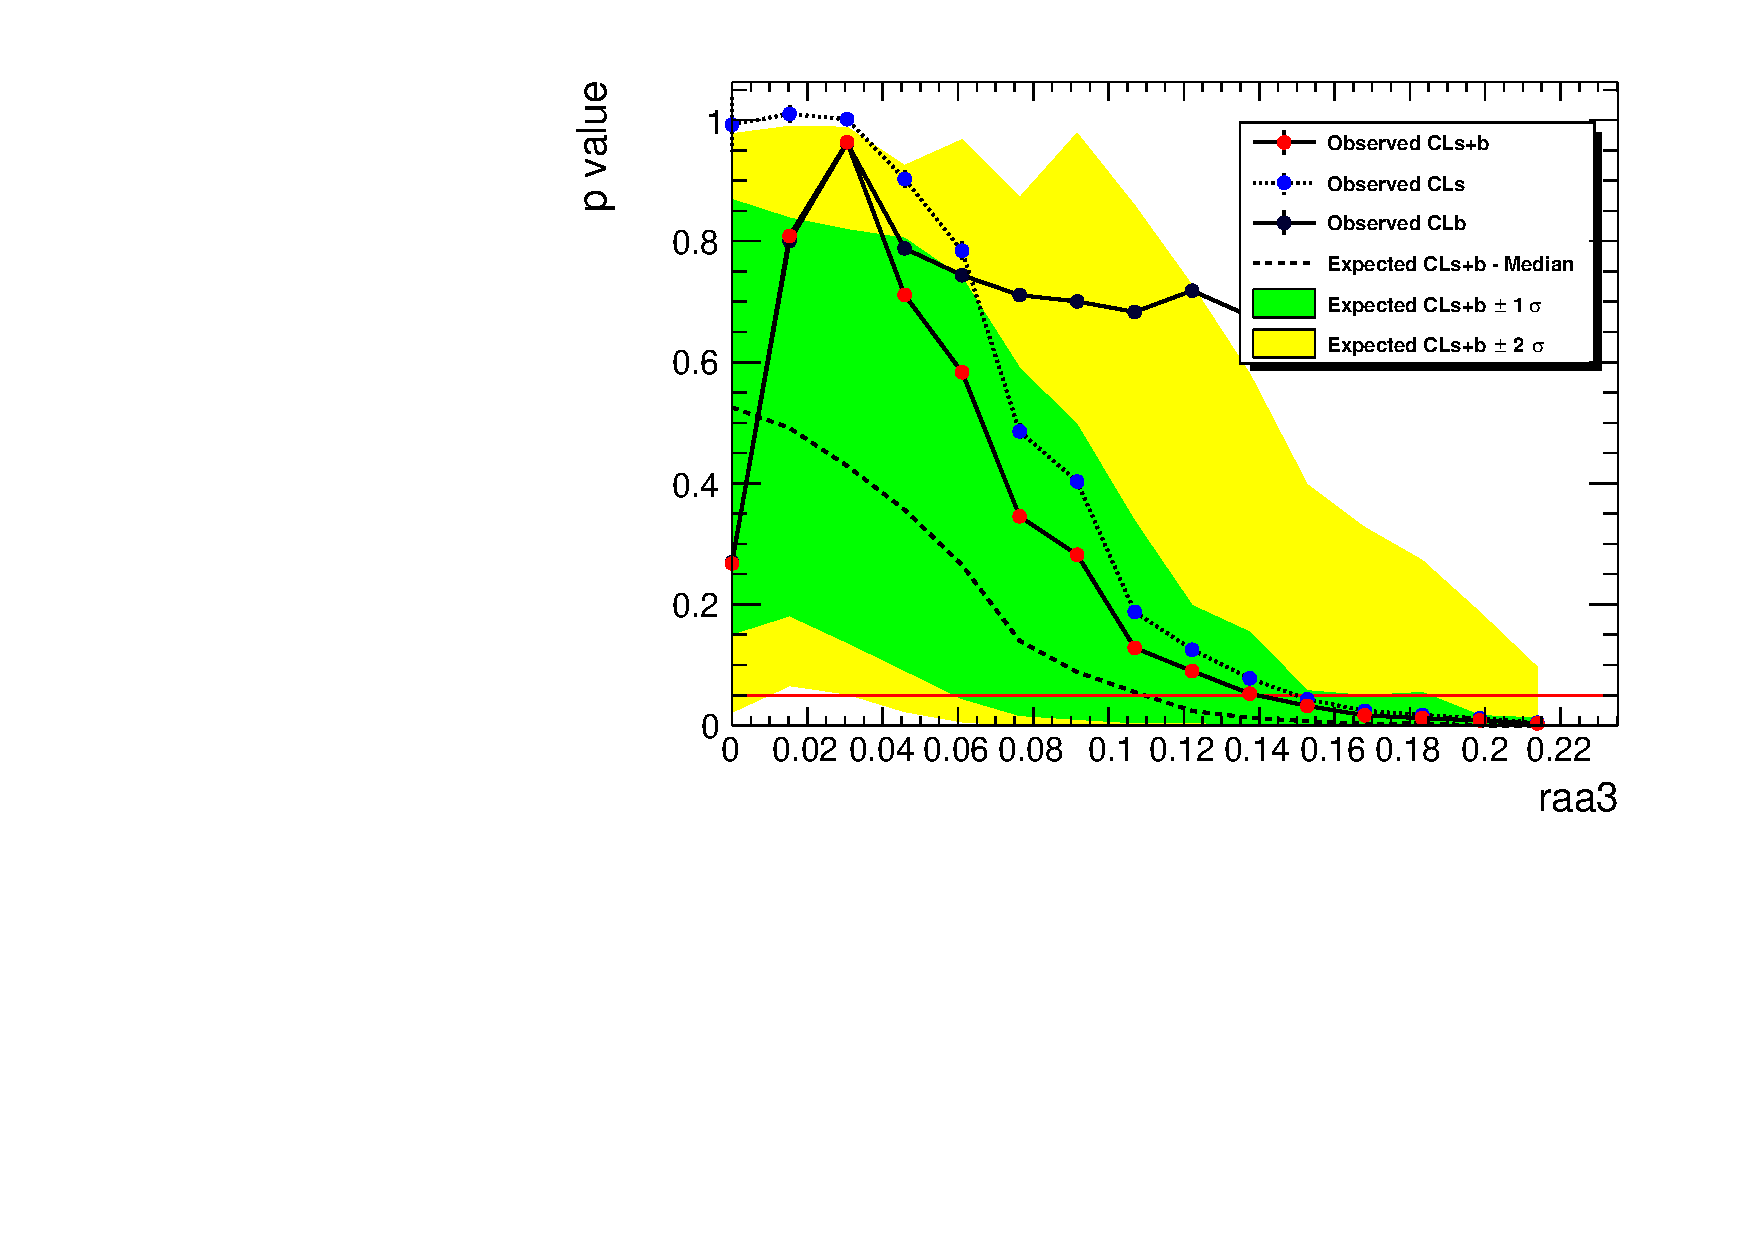
\includegraphics[width=0.49\textwidth]{Results/frequentist_x3raw_simple.pdf}
  \caption{Asymptotic scan (left) and frequentist scan (right) of the ratio of raw 3S yields in pp and PbPb collisions, based on the Feldman and 
     Cousins approach, giving the 95\% C.L. upper limit on $\RAA(\PgUc)$.}
  \label{fig:3SUL} 
\end{centering}
\end{figure}

\begin{figure}[h]
\begin{centering}       
  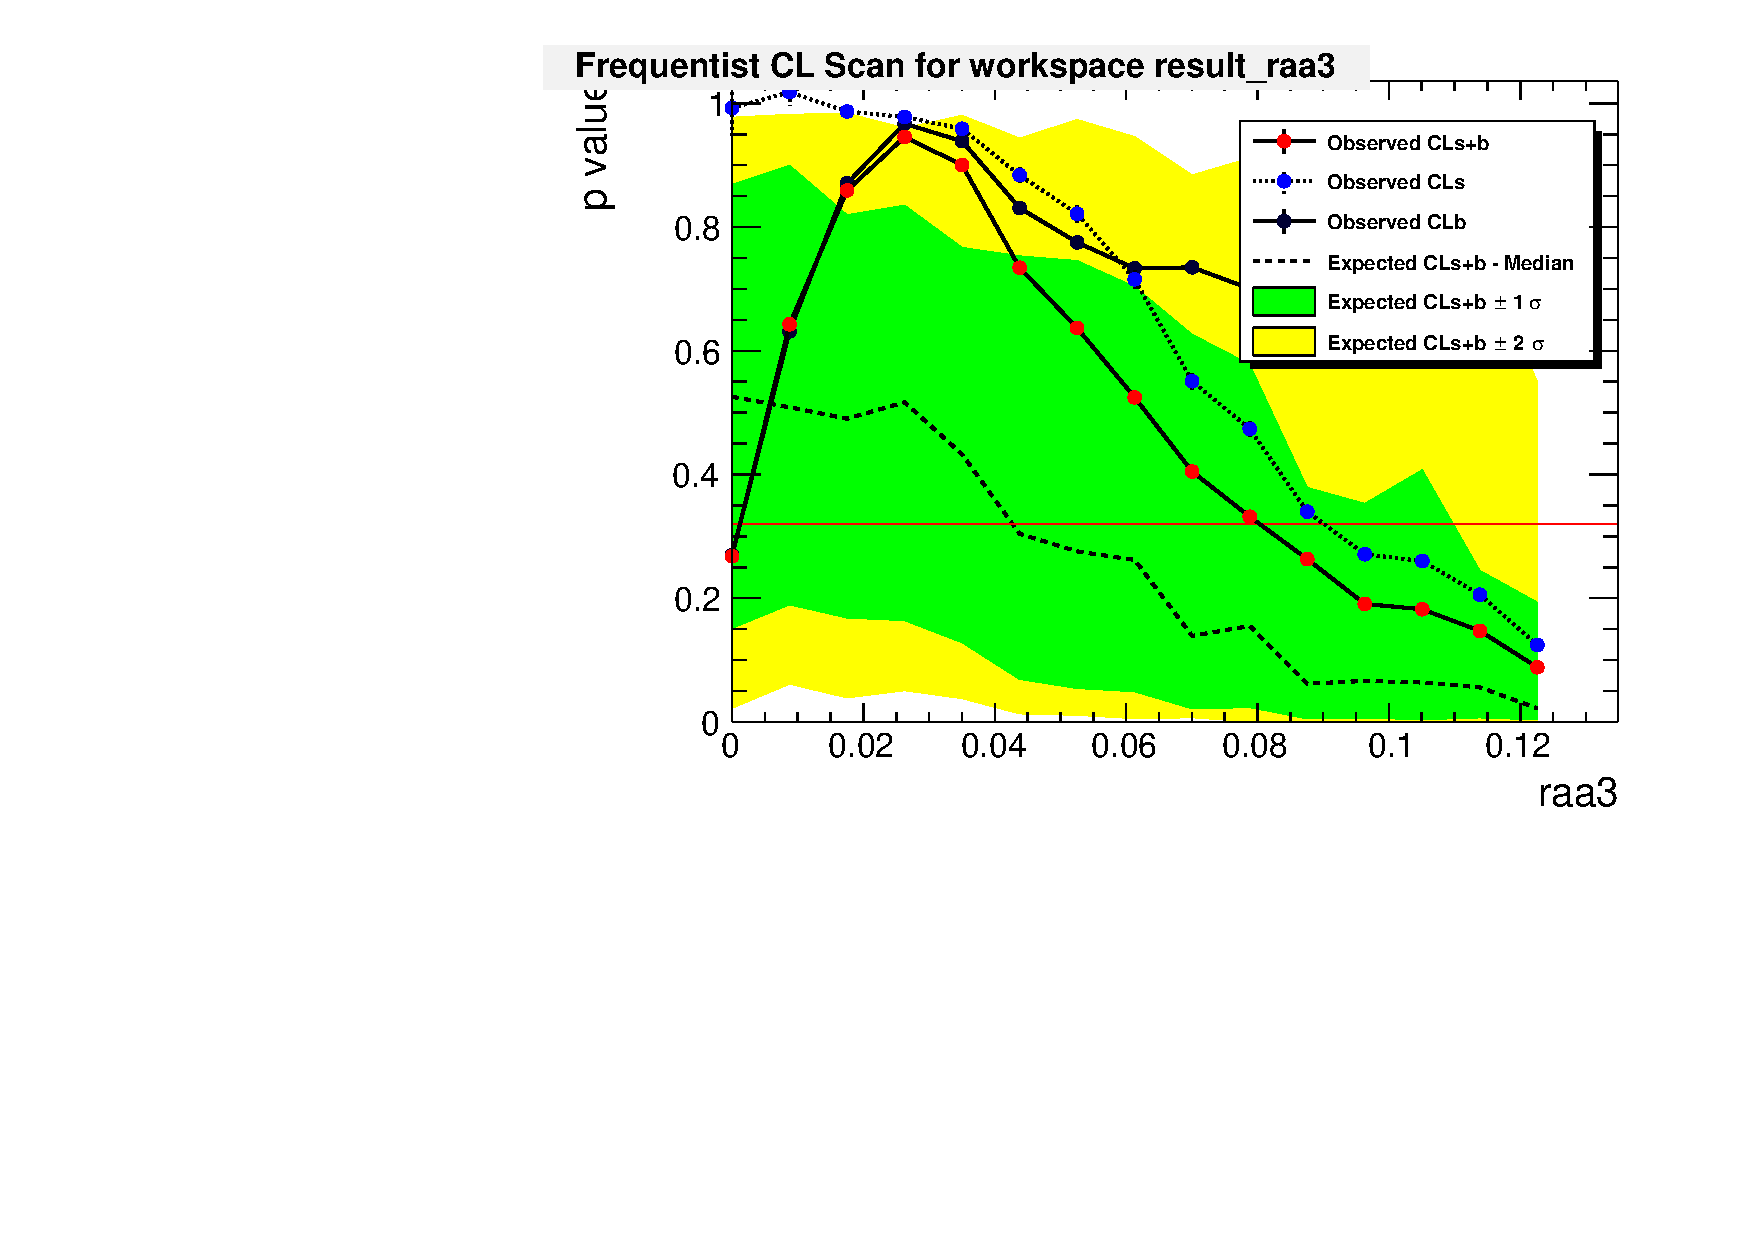
\includegraphics[width=0.49\textwidth]{Results/frequentist_x3raw_simple_68.pdf}
  \caption{Frequentist scan of the ratio of raw 3S yields in pp and PbPb collisions, based on the Feldman and Cousins approach, giving the 68\% C.L. upper limit on $\RAA(\PgUc)$.}
  \label{fig:3SUL_68} 
\end{centering}
\end{figure}

% \begin{figure}[h]
% \begin{centering}       
%   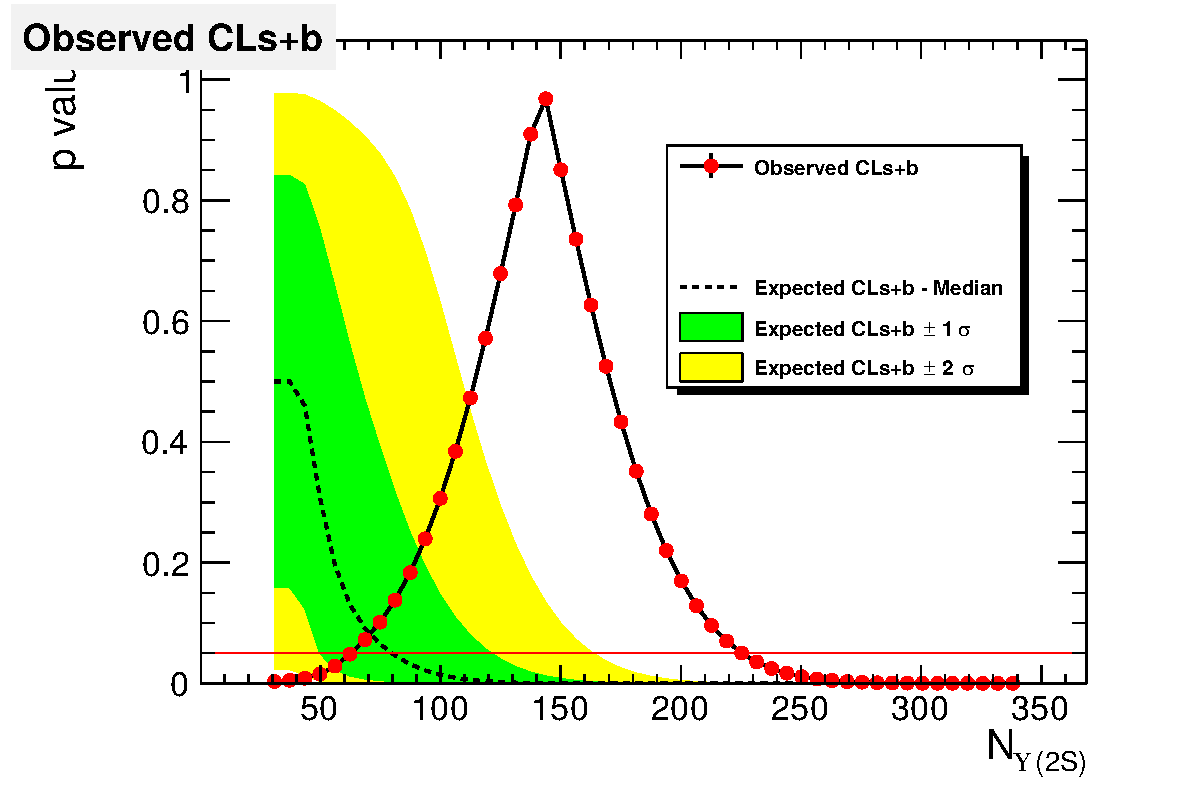
\includegraphics[width=0.8\textwidth]{Results/asymptotic_asimov_2S_simple.pdf}
%   \caption{Asymptotic scan of the 2S raw yield in PbPb based on the Feldman and Cousins approach.}
%   \label{fig:2SCI} 
% \end{centering}
% \end{figure}
\vfill\newpage
\subsection{68\% and 95\% confidence level intervals on \PgUb production\label{sec:limits2S}}

Similarly to what has been done for \PgUc, and because the PbPb yields of \PgUb{} are not very significant in most cases, we have determined 68\% and 95\% C.L. intervals
for the \RAA{} of the \PgUb. Following once again the Feldman-Cousins prescription, these intervals are actually upper limits in some cases, if the lower limit is 0.

The results with the nominal single muon cuts (4\,GeV on both muons) are given in Table~\ref{tab:2Stight}, using the frequentist calculation (see previous subsection). 
Intervals using other methods (asymptotic calculation, likelihood scan) are given in Section~\ref{sec:limits2S_tight} in the cross-checks section.
The results with the ``alternative'' single muon cuts (3.5\,GeV on one muon and 4\,GeV on the other) are also available, and they are presented in 
Section~\ref{sec:limits2S_alt}.

\begin{table}
\begin{center}
 \begin{tabular}{|c|c|c|c|c|}

\hline
Variable & Range & \RAA central value & 68\% & 95\% \\
\hline
\hline
$p_T$ & $[0,5]$ & 0.082 & $[0.031,0.115]$ & $[0.002,0.158]$ \\
$p_T$ & $[5,12]$ & 0.066 & $[0.020,0.109]$ & $[0,0.160]$ \\
$p_T$ & $[12,20]$ & 0.140 & $[0.102,0.241]$ & $[0.058,0.316]$ \\
\hline
$|y|$ & $[0,1.2]$ & 0.113 & $[0.063,0.137]$ & $[0.033,0.173]$ \\
$|y|$ & $[1.2,2.4]$ & 0.135 & $[0.0053,0.146]$ & $[0.012,0.195]$ \\

\hline
\end{tabular}
\end{center}
\caption{68\% and 95\% C.L. Feldman-Cousins intervals for the \PgUb}\label{tab:2Stight}
\end{table}

\vfill\newpage
\section{Summary}

The \PgUa, \PgUb\ and \PgUc\ mesons have been searched for in PbPb collisions, and compared to their yields in pp collisions at the same energy, 2.76 TeV. The \PgUa and \PgUb\ are suppressed by a factor of $\approx 2$ and 10, respectively, while the unobserved \PgUc\ corresponds to a suppression by a factor of 7.1, at 95\% confidence level. Though a strong centrality dependence of the suppression is observed for the \PgUa and \PgUb\ as a function of centrality, no noticeable dependence is observed, neither as a function of transverse momentum, nor as a function of rapidity. 

The \PgUc\ being not observed, an \RAA upper limit is derived, using the Feldman-Cousins prescription. Its result, together with the integrated \RAA values of the \PgUa and \PgUb\ are: 
\begin{eqnarray}
\RAA (\PgUa) & = & 0.425 \pm 0.024 \pm 0.034, \\
\RAA (\PgUb) & = & 0.116 \pm 0.028 \pm 0.013, \\
\RAA (\PgUc) & < & 0.014 {\rm \; at \; 95\% \; CL.} 
\end{eqnarray}
